En esta sección se detallarán los casos de uso y escenarios pertenecientes al subsistema de gestión de comentarios. La figura \ref{fig:casos_uso_subsistema_comentarios} muestra el diagrama de casos de uso de dicho subsistema.

\begin{figure}[h]
\centering
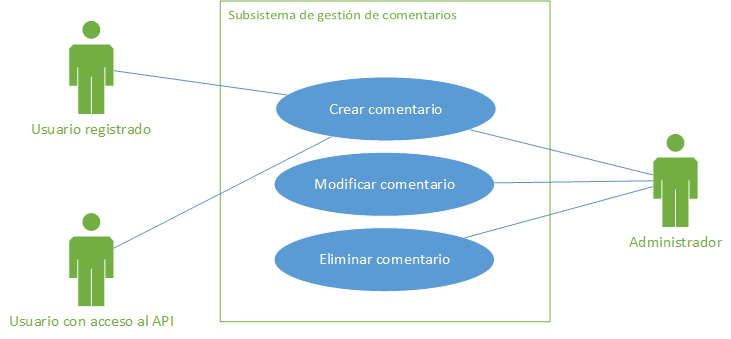
\includegraphics[width=\textwidth]{casos_uso_comentarios}
\caption{Diagrama de casos de uso del subsistema de gestión de comentarios}
\label{fig:casos_uso_subsistema_comentarios}
\end{figure}


\subsubsection{Caso de uso ``crear comentario''}
\begin{description}
\item[Descripción] El usuario quiere crear un nuevo comentario.
\item[Actores] Administrador, usuario registrado o usuario con capacidad de acceso al API.
\item[Precondiciones] Haber iniciado sesión en el sistema.
\item[Escenario principal] \hfill
						 	\begin{enumerate}
							\item El usuario accede a la entrada del blog o al debate en el que quiere crear el comentario.
							\item El usuario escribe su comentario.
							\item Pulsa el botón de para guardar su comentario.
							\item El sistema guarda el comentario y lo hace visible al resto de usuarios.
							\end{enumerate}
\item[Escenario alternativo 1] Comentario en un  debate cerrado.
							\begin{enumerate}
							\item El usuario accede al debate en el que quiere crear el comentario.
							\item El sistema no mostrará opciones para que el usuario cree un comentario.
							\end{enumerate}
\end{description}


\subsubsection{Caso de uso ``modificar comentario''}
\begin{description}
\item[Descripción] El administrador desea modificar el contenido de un comentario realizado por un usuario.
\item[Actores] Administrador.
\item[Precondiciones] Haber iniciado sesión en el sistema.
\item[Escenario principal] \hfill
						 	\begin{enumerate}
							\item El usuario accede a la entrada del blog o al debate en el que se encuentra el comentario a modificar.
							\item El administrador localiza el comentario y pulsa el botón modificar.
							\item El administrador introduce el texto que crea conveniente y pulsa el botón guardar.
							\item El sistema actualiza el contenido del comentario modificado.
							\end{enumerate}
\end{description}


\subsubsection{Caso de uso ``eliminar comentario''}
\begin{description}
\item[Descripción] El administrador desea eliminar un comentario realizado por un usuario.
\item[Actores] Administrador.
\item[Precondiciones] Haber iniciado sesión en el sistema.
\item[Escenario principal] \hfill
						 	\begin{enumerate}
							\item El usuario accede a la entrada del blog o al debate en el que se encuentra el comentario a eliminar.
							\item El administrador localiza el comentario y pulsa el botón eliminar.
							\item El sistema elimina el comentario y deja de mostrarlo.
							\end{enumerate}
\end{description}